\chapter{設計}
\label{chap:function}

本章では, まず本研究で作成した Delta Smile Facial Survey Analyzerシステムの
設計概要について説明する.
その後, データ収集機能における各モジュールと, データ分析機能における各モジュールの
詳細について説明する.

\section{本システムの設計概要}
本研究で作成したDelta Smile Facial Survey Analyzer(以下DSFSA)は,
素材動画から笑顔動画データおよび画像処理結果を保存したCSVデータの作成,
ユーザーの笑顔動画データの作成, および画像処理結果を保存したCSVデータを使用して,
データベースにあるCSVデータと演算を行い, 選ばれた動画データに対してユーザーに順位づけをしてもらう
laptop上で動くデータ収集・分析用システムである.
本システムのシステム構成図を\ref{fig:system_architecture}に示す.

\begin{figure}[htbp]
    \begin{center}
       \fbox{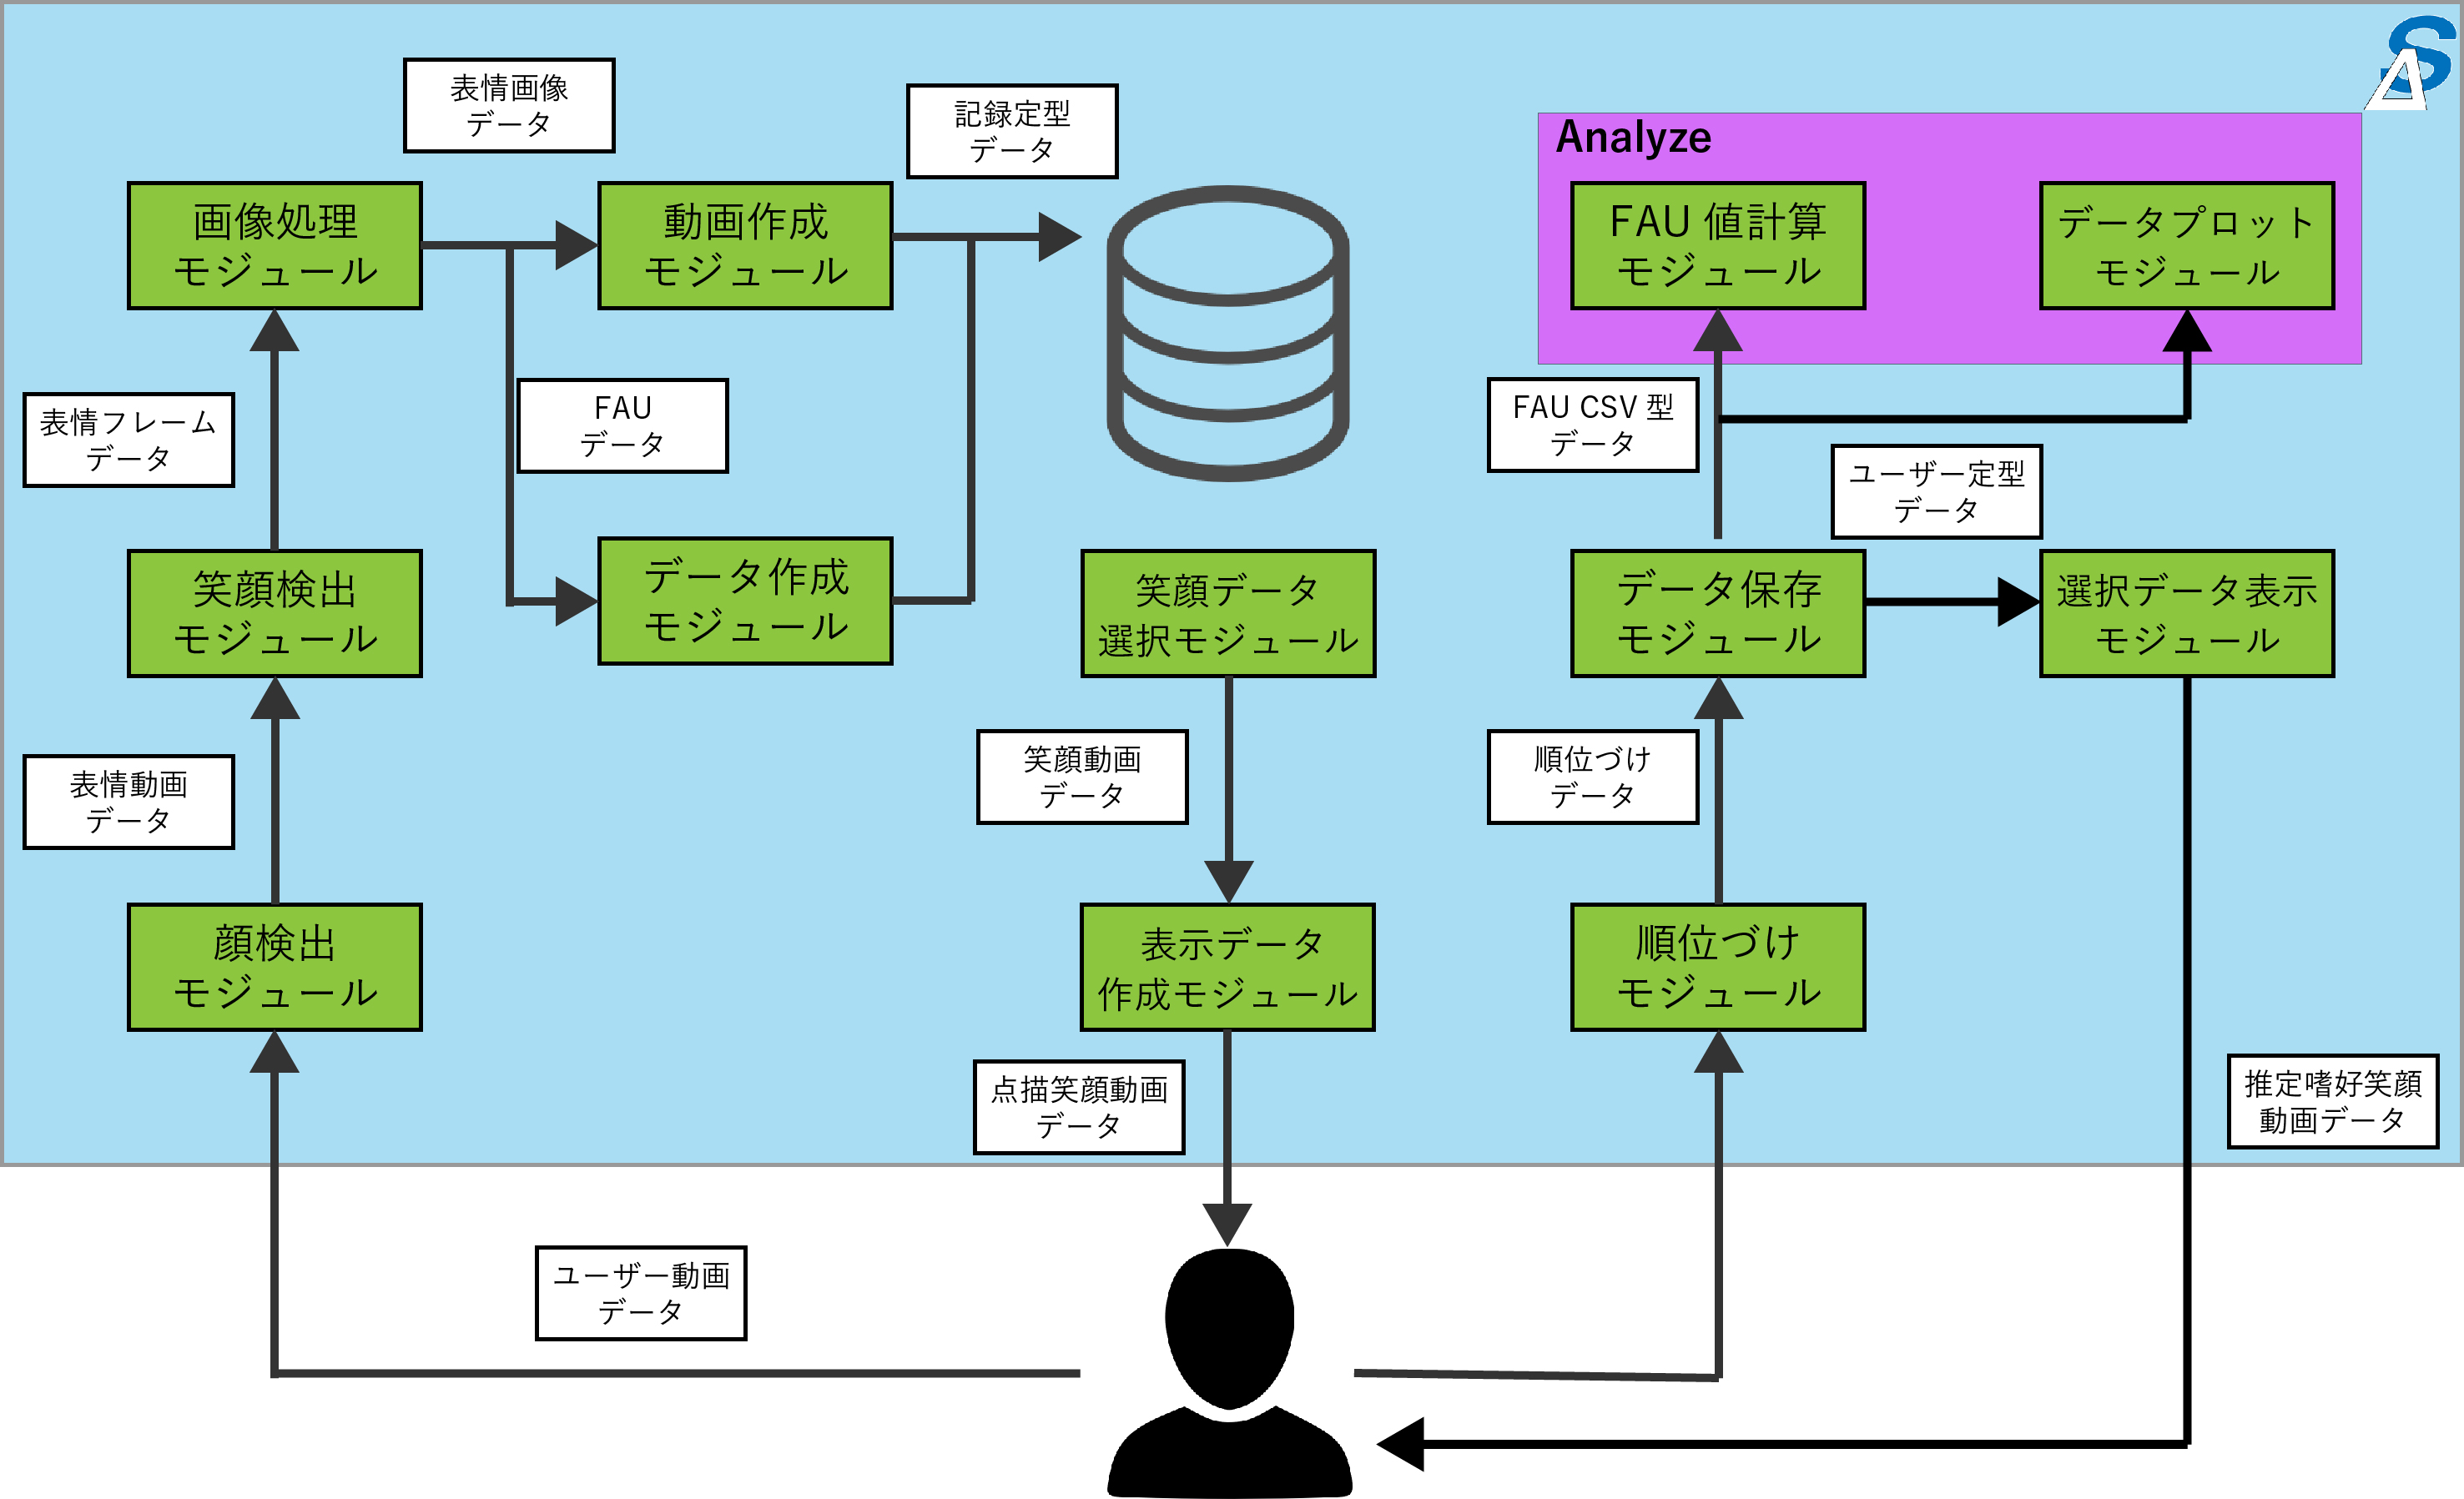
\includegraphics[width=140mm,bb=0 0 2953 1797]{system_architecture.jpg}}
    \end{center}
    \caption{システム構成図}
    \label{fig:system_architecture}
\end{figure}

\section{データ収集機能}
\subsection{顔検出モジュール}
\subsection{笑顔検出モジュール}
\subsection{画像処理モジュール}
\subsection{データ作成モジュール}
\subsection{笑顔データ選択モジュール}
\subsection{表示データ作成モジュール}
\subsection{順位づけモジュール}
\subsection{データ保存モジュール}
\subsection{選択データ表示モジュール}

\section{データ分析機能}
\subsection{FAU値計算モジュール}
\subsection{データプロットモジュール}
\section{まとめ}
